\documentclass[tikz]{standalone}
\usetikzlibrary{intersections}
\usepackage{xparse}
\colorlet{curveZero}{gray!85}
\colorlet{curveOne}{blue!60}
\definecolor{curveOneColor}{rgb}{.6,0,0}
\colorlet{curveTwo}{brown!50!gray}
\colorlet{curveThree}{green!40!gray}
\colorlet{curveFour}{red!50!gray}
\NewDocumentCommand\DrawDotInPlot{O{}mmO{}}%
{%
\fill[gray!15,draw=gray] (axis cs:{#2},{#3}) circle [radius=1.6pt] node[above,black,#4] {\(#1\)};%
}%
\NewDocumentCommand\DrawDot{O{}mmO{}}%
{%
\fill[gray!20,draw=gray] ({#2},{#3}) circle (1.6pt) node[above,black,#4] {\(#1\)};%
}%
\NewDocumentCommand\DrawNode{O{}m}%
{%
\fill[gray!20,draw=gray] (#2) circle (1.6pt) node[above,black] {\(#1\)};%
}%
\NewDocumentCommand\DrawDotThreeD{O{}mmmO{}}%
{%
\fill[gray!20,draw=gray] ({#2},{#3},{#4}) circle (1.6pt) node[above,black,#5] {\(#1\)};%
}%
\colorlet{axisColor}{gray!50}
\tikzstyle{shapeZero}=[fill=curveZero,opacity=.4]
\tikzstyle{shapeOne}=[fill=curveOne,opacity=.4]
\tikzstyle{shapeTwo}=[fill=curveTwo,opacity=.4]
\tikzstyle{shapeThree}=[fill=curveThree,opacity=.4]
\tikzstyle{groupElementLabel}=[minimum size=2.4em]
\tikzstyle{groupElement}=[minimum size=2.4em,shapeZero,draw=curveZero]
\tikzstyle{cosetOne}=[minimum size=2.4em,shapeOne,draw=curveOne]
\tikzstyle{cosetTwo}=[minimum size=2.4em,shapeTwo,draw=curveTwo]


\begin{document}
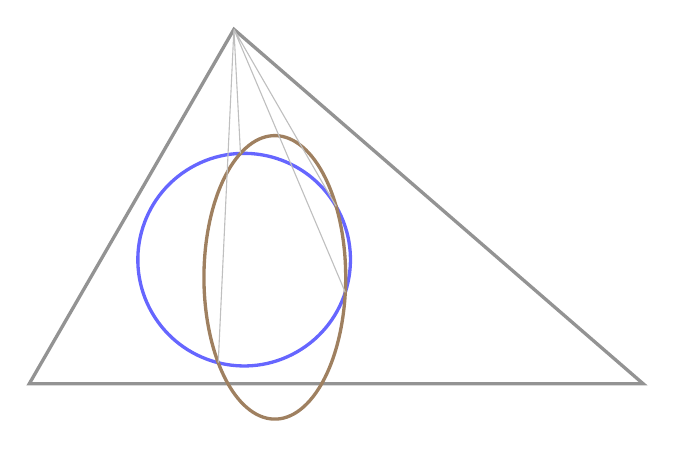
\begin{tikzpicture}[scale=3]
\draw[curveZero,very thick] 
({cos(90)},{sin(90)}) -- 
({cos(90+120)},{sin(90+120)}) -- 
({2*cos(90+2*120)},{sin(90+2*120)}) -- cycle;
\draw[curveOne,very thick,name path=Bellipse] ({.5*cos(90)+.5*cos(90+2*120)},{.5*sin(90)+.5*sin(90+2*120)}) arc (30:390:.45);
\draw[curveTwo,very thick,name path=Cellipse] ({.5*cos(90)+.5*cos(90+2*120)},{.5*sin(90)+.5*sin(90+2*120)}) arc (30:390:.3 and .6);
\draw [axisColor, name intersections={of=Bellipse and Cellipse}]
(intersection-1) -- ({cos(90)},{sin(90)}) 
(intersection-2) -- ({cos(90)},{sin(90)}) 
(intersection-3) -- ({cos(90)},{sin(90)}) 
(intersection-4) -- ({cos(90)},{sin(90)}); 
\end{tikzpicture}
\end{document}
